\documentclass[justified]{article}

\usepackage{amsmath, amsfonts, amssymb, amsthm}
\usepackage[margin=1.1in]{geometry}
\usepackage{hyperref}

\usepackage{float}
\usepackage{microtype}
\usepackage{mathpazo}
\usepackage{tikz}

\hypersetup{
    colorlinks=true,
    linkcolor=blue,
    filecolor=magenta,
    urlcolor=blue,
}

\urlstyle{same}

\tikzstyle{circleblock} = [draw, fill=white, circle, inner sep=0]

\begin{document}
  \title{Data Preprocessing Methods for Noise-Resistant CNNs}
  \author{Rowen Hunter, Eero Gallano, Jonathan Lee}
  \date{\today}
  \maketitle

  \section{Problem Statement and Background}
  % Motivation, related work, summary of contribution, results

  \section{Approach}
  % Assumptions, definitions, objective

  \subsection{Data Augmentation}

  In order for our classifier to generalize, it needs to be trained on a varied and

  \subsection{Models}

  Existing deep neural networks for image classification, such as ResNet50, already offer very good feature extraction for generic tasks.
  Therefore, we used

  In order to

  \begin{figure}[H]
    \centering
    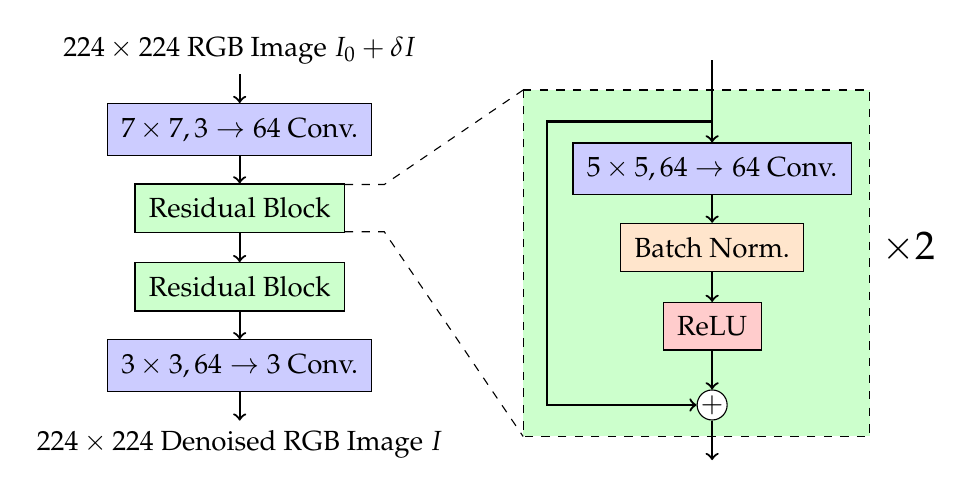
\begin{tikzpicture}
      \node (input) at (0, 0) {$224 \times 224$ RGB Image $I_0 + \delta I$};
      \node[draw, fill=blue!20, inner sep=5pt] (conv7x7) at (0, -1) {$7 \times 7, 3 \to 64$ Conv.};
      \node[draw, fill=green!20, inner sep=5pt] (resid1) at (0, -2) {Residual Block};
      \node[draw, fill=green!20, inner sep=5pt] (resid2) at (0, -3) {Residual Block};
      \node[draw, fill=blue!20, inner sep=5pt] (conv3x3) at (0, -4) {$3 \times 3, 64 \to 3$ Conv.};
      \node (output) at (0, -5) {$224 \times 224$ Denoised RGB Image $I$};
      \fill[green!20] (3.6, -0.5) rectangle (8, -4.9);

      \node (blockin) at (6, 0) {};
      \node[draw, fill=blue!20, inner sep=5pt] (conv5x5) at (6, -1.5) {$5 \times 5, 64 \to 64$ Conv.};
      \node[draw, fill=orange!20, inner sep=5pt] (batchnorm) at (6, -2.5) {Batch Norm.};
      \node[draw, fill=red!20, inner sep=5pt] (relu) at (6, -3.5) {ReLU};
      \node (blockout) at (6, -5) {};
      \node at (8.5, -2.5) {\Large $\times 2$};
      \node[circleblock] (sum) at (6, -4.5) {$+$};

      \draw[->, thick] (input) -- (conv7x7);
      \draw[->, thick] (conv7x7) -- (resid1);
      \draw[->, thick] (resid1) -- (resid2);
      \draw[->, thick] (resid2) -- (conv3x3);
      \draw[->, thick] (conv3x3) -- (output);

      \draw[->, thick] (blockin) -- (conv5x5);
      \draw[->, thick] (conv5x5) -- (batchnorm);
      \draw[->, thick] (batchnorm) -- (relu);
      \draw[->, thick] (relu) -- (sum);
      \draw[->, thick] (sum) -- (6, -5.2);
      \draw[dashed] (3.6, -0.5) -- (8, -0.5) -- (8, -4.9) -- (3.6, -4.9) -- (3.6, -0.5);
      \draw[dashed] (resid1.east) ++ (0, 0.3) -- ++(0.5, 0) -- (3.6, -0.5);
      \draw[dashed] (resid1.east) ++ (0, -0.3) -- ++(0.5, 0) -- (3.6, -4.9);
      \draw[->, thick] (6, -0.9) -- (3.9, -0.9) -- (3.9, -4.5) -- (sum);
    \end{tikzpicture}
    \caption{
      Denoising network architecture.
      All convolutional blocks use stride 1 and padding such that the spatial dimensions are preserved.
    }
  \end{figure}

  The denoinsing network uses mean squared error (MSE) as its loss function.
  We can use the MSE to estimate the peak signal-to-noise ratio (PSNR), a nonnegative quantity measured in decibels (dB) that increases as $I \to I_0$ (\textit{i.e.}, the denoising network undoes the perturbation $\delta I$) and goes to zero when the MSE is maximized.
  \begin{equation}
    \begin{split}
      \mathsf{MSE}(I_0, I) &= \frac{1}{MN} \sum_{(x, y, c)} \left(I_0(x, y, c) - I(x, y, c)\right)^2 \\
      \mathsf{PSNR}(I_0, I) &= 10 \log_{10} \left(\frac{3^2}{\mathsf{MSE}(I_0, I)}\right)
    \end{split}
  \end{equation}

  \begin{enumerate}
  \item Augment the dataset with rotated, shifted, scaled (input perturbations)
  \item Add noise (AWGN, one-shot, patches), train denoising network
  \item ResNet-like architecture
  %+ Additive white Gaussian noise layers?
  % denoising layers?
  % compression?
  % ensembles
  % \item FGSM-generated samples
  \end{enumerate}

  \section{Results}

  \section{Tools}

  We implemented our models in \href{https://pytorch.org/}{PyTorch}, a popular deep learning framework that offers standardized, performant implementations of learning primitives such as tensors, fully connected and convolutional layers, optimizers, and loss functions.

  \section{Lessons Learned}

  Selecting a bad learning rate can cause a model to fail to make full use of its capacity.
  Na\"{i}ve schemes like an exponentially decaying learning rate did not work particularly well because it's hard to tell \textit{a priori} what the base learning rate and the decay rate should be.
  % Adaptive schemes, such as the one-cycle learning rate policy, tended to work better because

  \section{Team Contributions}

  \begin{itemize}
  \item
    Jonathan Lee built, trained, and evaluated the denoising network.
    He wrote the training script and designed the perturbations.
    Estimated contribution: 35\%.
  \end{itemize}
\end{document}
